\chapter{Simulation \& Experimental Results}
The previous chapters were concerned with algorithm translation and system design. This chapter presents the methodology and results of the system simulation. The designed algorithm and system are implemented using MATLAB.

\section{System Simulation}
The system is implemented using MATLAB, as explained in Section 4.3. A sine, square and sawtooth signals with different frequencies and phase differences are used as test signals to simulate the performance of the implemented system. A delay object is introduced in the system to model the transmission process effectively. The simulation uses MATLAB TimeScope objects to display the time-domain representation of the input, transmitted, reconstructed, and error signals. The system uses channel models (AWGN, Rician) to add noise to the transmitted signal and simulate real-world scenarios. Fig. \ref{sim_output} shows the output of system simulation. The effect of interpolation by the Filter Bank is seen by observing the frequency spectrum of the input and transmitted signals shown in Fig. \ref{spec}. The input and reconstructed signals are normalized and are used to calculate the mean error rate of the system in various conditions. 

\begin{figure}[htpb]
\centering
\begin{tabular}{cc}
  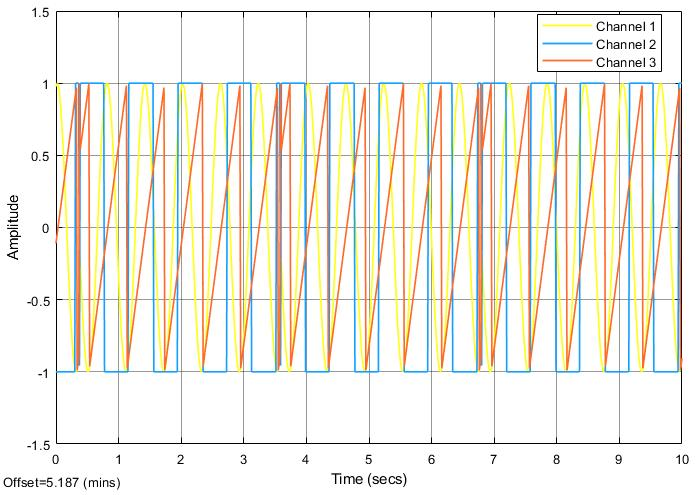
\includegraphics[width=80mm]{original_signal.jpg} & 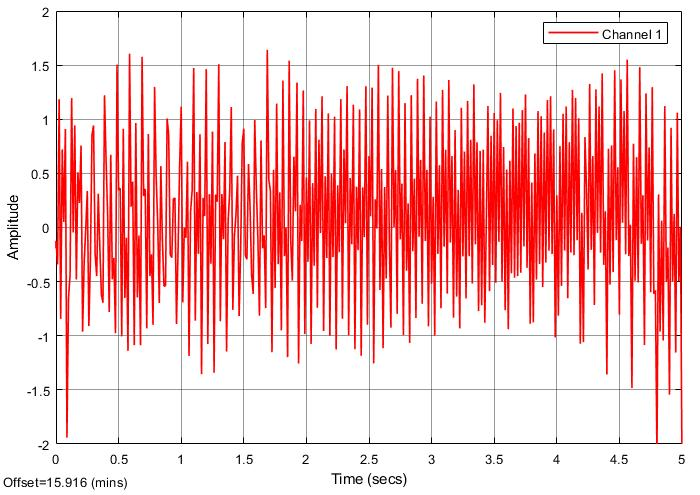
\includegraphics[width=80mm]{transmitted_signal.jpg} \\
(a) Original Signals  & (b) Transmitted Signal  \\[8pt]
 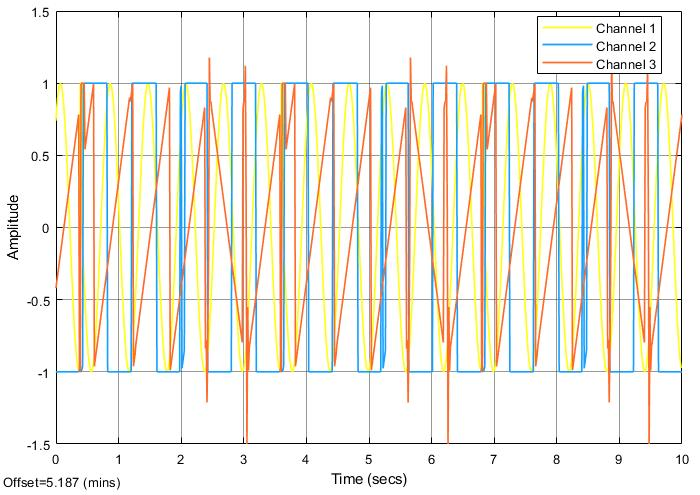
\includegraphics[width=80mm]{reconstructed_signal.jpg} & 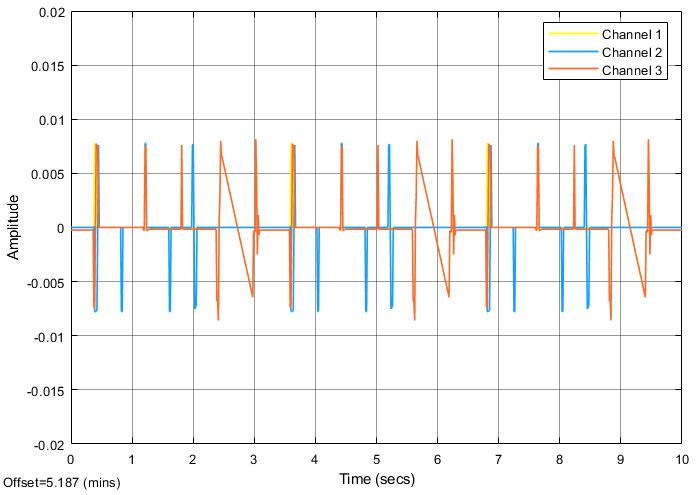
\includegraphics[width=80mm]{error_signal.jpg} \\
(c) Reconstructed Signals  & (d) Error Signals  \\[8pt]
\end{tabular}
\caption{Output of System Simulation.}
\label{sim_output}
\end{figure}

\begin{figure}[htpb]
\centering
\begin{tabular}{cc}
  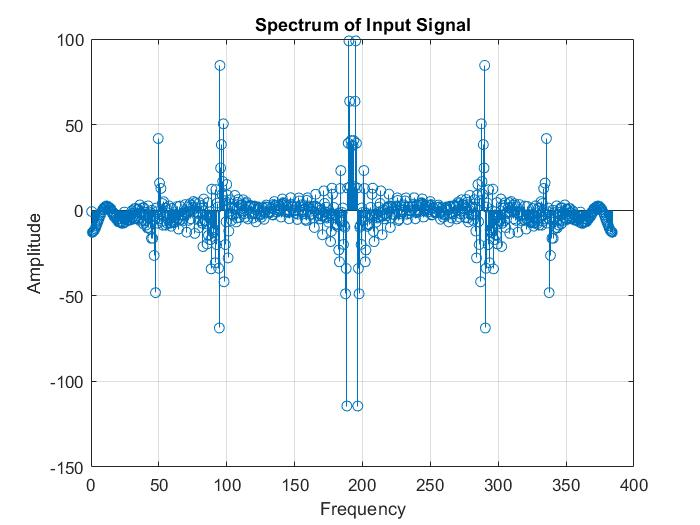
\includegraphics[width=80mm]{Input_Spectrum.jpg} & 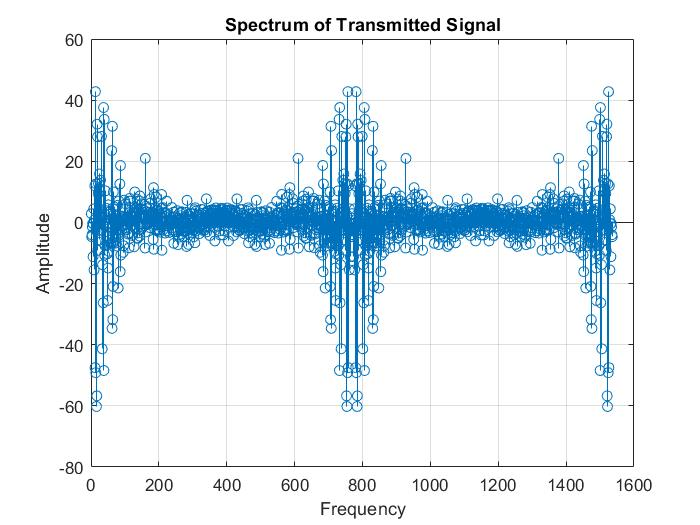
\includegraphics[width=80mm]{Transmitted_Spectrum.jpg} \\
(a) Input Signal Spectrum  & (b) Transmitted Signal Spectrum  \\[8pt]
\end{tabular}
\caption{Effect of Interpolation on Spectrum of Signal $(M = 4)$.}
\label{spec}
\end{figure}

\section{Evaluation Metrics}
The simulation uses Mean Squared Error (MSE) of the normalized input and reconstructed signals to evaluate the implemented system. The MSE of the system is given by: 
\[
MSE = \frac{1}{n}\sum_{i=1}^{n}(X_i-\hat{X}_i)^2
\]
where, \\
${n}$ = number of data points \\
$X_{i}$ = Normalized Input Signal \\
$\hat{X}_{i}$ = Normalized Reconstructed Signal

\newpage
The system was tested with different types of wavelets as given in Table \ref{wlets}. Table \ref{tab:sim} shows the MSE values of the system for various Mother Wavelets under different channel conditions for a Signal-to-noise ratio (SNR) of -20 dBW (Without any channel, AWGN, and Rician). The Designed wavelet filter showcases an improvement of approximately 70 \% compared to other Wavelet families.

\begin{itemize}
    \item The Additive White Gaussian Noise (AWGN) channel is based on the Information Theory and is used to model the effect of various random processes in nature. It is a simple mathematical model which is useful for gaining insight into the underlying behavior of a system before these other phenomena such as fading, interference, non-linearity, or dispersion are considered.
    \item The Rician Fading channel is a model which characterizes multi-path fading and interference under Line of Sight (LoS) conditions. Rician fading occurs when one of the signal propagation paths is much stronger than the others and is characterized by the Rician distribution.
\end{itemize}

\begin{table}[hptb]
  \centering
  \begin{tabular}{|c|c|c|c|c|}
  \hline
    \multicolumn{4}{|c|}{Mean Error Rate} \\
    \hline
    & \multicolumn{3}{c|}{Channel Model} \\
    \hline
    Wavelet Family & Without Channel & AWGN & Rician Fading \\
    \hline
    \multicolumn{1}{|c|}{Designed Wavelet Filters} & 1.41 x $10^{-8}$ & 0.009215 & 0.0380 \\
    \hline
    \multicolumn{1}{|c|}{Haar} & 4.35 x $10^{-8}$ & 0.012177 & 0.0437   \\
    \hline
    \multicolumn{1}{|c|}{Daubechies} & 2.34 x $10^{-8}$ & 0.009020 & 0.0411 \\
    \hline
    \multicolumn{1}{|c|}{Symlets} & 2.75 x $10^{-8}$ & 0.010338 & 0.0484  \\
    \hline
    \multicolumn{1}{|c|}{Biorthogonal} & 3.16 x $10^{-8}$ & 0.013067 & 0.0455\\
    \hline
  \end{tabular}
\caption{\label{tab:sim}Mean Error Rate of the System for SNR = $-20$ dBW}
\end{table}

Table \ref{tab:error_awgn} shows the MSE values for the Proposed system that uses DWT-based Filter banks for different SNR values through an AWGN channel. These values are compared with a corresponding Conventional system implemented using FFT-based filter banks. The proposed system outperforms the conventional system by a factor of approximately $10^{-4}$. Fig. \ref{fig:error_plot_awgn} shows the MSE v/s SNR plot for the Proposed and Conventional system for an AWGN channel.

\begin{table}[htpb]
    \centering
    \caption{Mean Error Rate of the System for AWGN Channel.}
    \begin{tabular}{|c|c|c|}
    \hline
    \multicolumn{3}{|c|}{Mean Error Rate} \\
    \hline
       SNR (dB)  & Proposed system & Conventional system \\
       \hline
        -50 & 1.02 & 1.7982 \\
         \hline
         -30 & 0.042634 & 0.6528\\
         \hline
         -20 & 0.002215 & 0.1929\\
         \hline
         -5 & 0.000165 & 0.00807\\ 
         \hline 
         10 & 0.000023 & 0.00087\\ 
         \hline
         20 & 0.0000012 & 0.00042\\
         \hline 
         30 & 1.23 x $10^{-8}$ & 9.1590 x $10^{-5}$\\
         \hline
    \end{tabular}
    \label{tab:error_awgn}
\end{table}

\begin{table}[htpb]
    \centering
    \begin{tabular}{|c|c|c|c|c|c|}
    \hline
    \multicolumn{6}{|c|}{Mean Error Rate} \\
    \hline
        SNR (dBW) & Proposed system & Haar & Symlets & Daubechies & Biorthogonal  \\
        \hline
         -50 & 1.02 & 2.4277 & 2.18552 & 2.075572 & 2.054686\\
        \hline
        -30 & 0.042634 & 1.20599 & 0.33654 & 0.352911 & 0.35962\\
        \hline
        -20 & 0.002215 & 0.012177 & 0.019020 & 0.009020 & 0.013067 \\
        \hline
         -5 & 0.000165 & 0.00169 & 0.000597 & 0.000352 & 0.000447\\
        \hline
         10 & 0.000023 & 0.00034 & 0.00025 & 0.00017 & 0.000026\\
        \hline
         20 & 0.0000012 & 0.000098 & 0.000021 & 0.000012 & 0.000017\\
        \hline
        30 & 1.23 x $10^{-8}$ & 0.0000027 & 0.000011 & 1.9 x $10^{-6}$ & 2.3 x $10^{-6}$ \\
        \hline
    \end{tabular}
    \caption{Mean Error Rate of the System for various Mother Wavelets.}
    \label{tab:error_awgn_wavelets}
\end{table}

Table \ref{tab:error_awgn_wavelets} shows the MSE of the system for various values of SNR and Mother Wavelets for an AWGN channel model. From the plots shown in Fig. \ref{fig:error_plot_wavelets}, we can see that the proposed system performs better than most Wavelet families by a factor of approximately $10^{-4}$ for SNR values greater than -10 dBW. The performance of the Daubechies family of Wavelets is most comparable to that of the Designed wavelet filters.

% \vspace{15mm}

\begin{figure}[htpb]
    \centering
    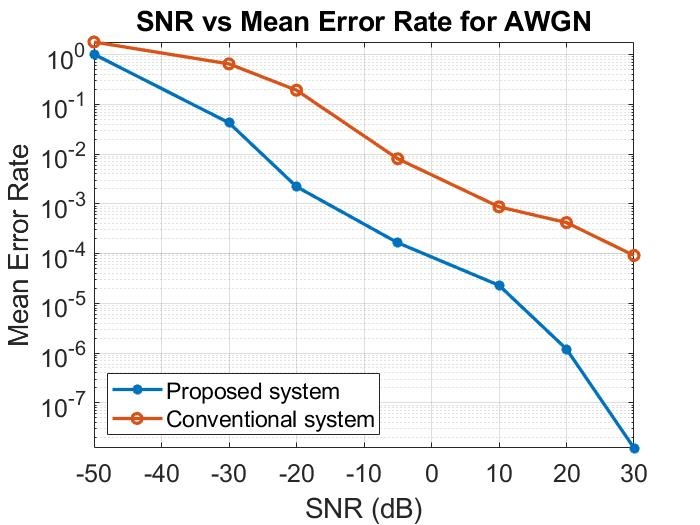
\includegraphics[width=120mm]{error_rate_awgn_v3.jpg}
    \caption{SNR v/s Mean Error Rate plot for AWGN Channel.}
    \label{fig:error_plot_awgn}
\end{figure}

\begin{figure}[htpb]
\centering
\begin{tabular}{c}
  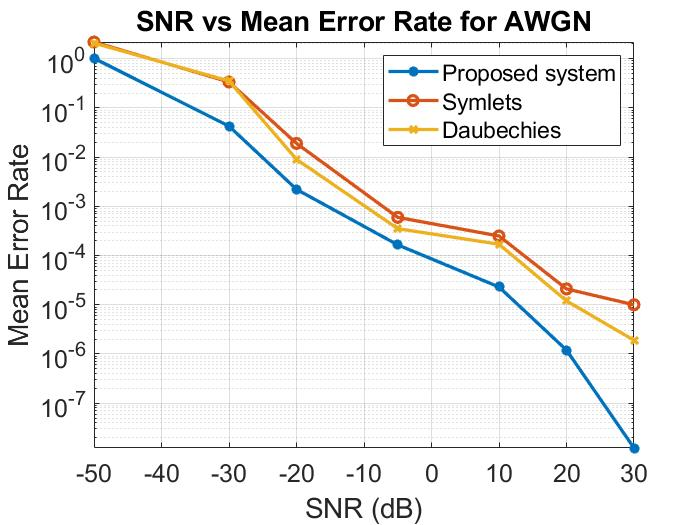
\includegraphics[width=100mm]{error_rate_wavelets_db.jpg} \\
  \vspace{10mm}
  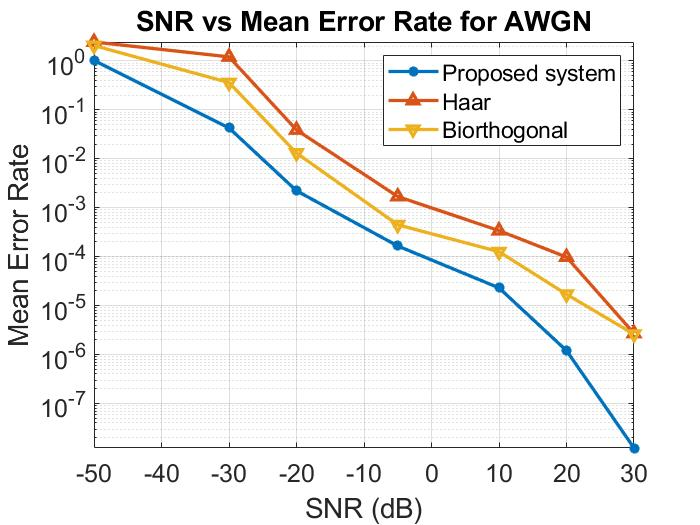
\includegraphics[width=100mm]{error_rate_wavelets.jpg} \\
\end{tabular}
\caption{SNR v/s Mean Error Rate plot for various Mother Wavelets.}
\label{fig:error_plot_wavelets}
\end{figure}

\newpage

\chapter{Experimental Results}

\section{Implementation using MATLAB HDL Coder}
This section explores the implementation of the designed system using the HDL Coder Toolbox in MATLAB. The HDL Coder facilitates the development and verification of hardware designs and automatically generates synthesizable RTL code to target specific FPGAs. The toolbox converts the input MATLAB function to work with Fixed-point data, after which it is converted to VHDL code. The user selects the target hardware and language as per requirements. \par
The HDL code generation for the system is done using 2 MATLAB functions for the transmitter and receiver, respectively. The work redefines the functions for dwt \cite{dwt} and discrete convolution to ensure compatibility with the toolbox. The designed filters are imported, and the system is implemented as per the block diagram. The functions designed for Generic Xilinx FPGAs perform 8-point dwt and idwt using persistent variable registers in MATLAB. For the HDL Test Bench, the system uses two audio signals and one chip signal for simulation. The work uses audio signals derived from the \textit{OpenSpeechRepository} based on Harvard Sentences \cite{speech}. These audio signals have a sample rate of 8 kHz and have a duration of 30 s, with a delay of 5 s introduced to the system. Based on the output of the Test Bench, it is inferred the audio signals are perfectly reconstructed and are clearly audible. The MSE of the system was 3.619 x $10^{-6}$. Fig. \ref{fig:test_bench_error} shows the Normalized Error Signals for the Test Bench audio signals. Fig. \ref{fig:hdl} shows the output screenshot of the Workflow Advisor of the HDL Coder in MATLAB. Fig. \ref{fig:rtl_transmitter} shows the RTL Schematic of the Transmitter generated using the VHDL code in Xilinx ISE.

\begin{figure}[htpb]
    \centering
    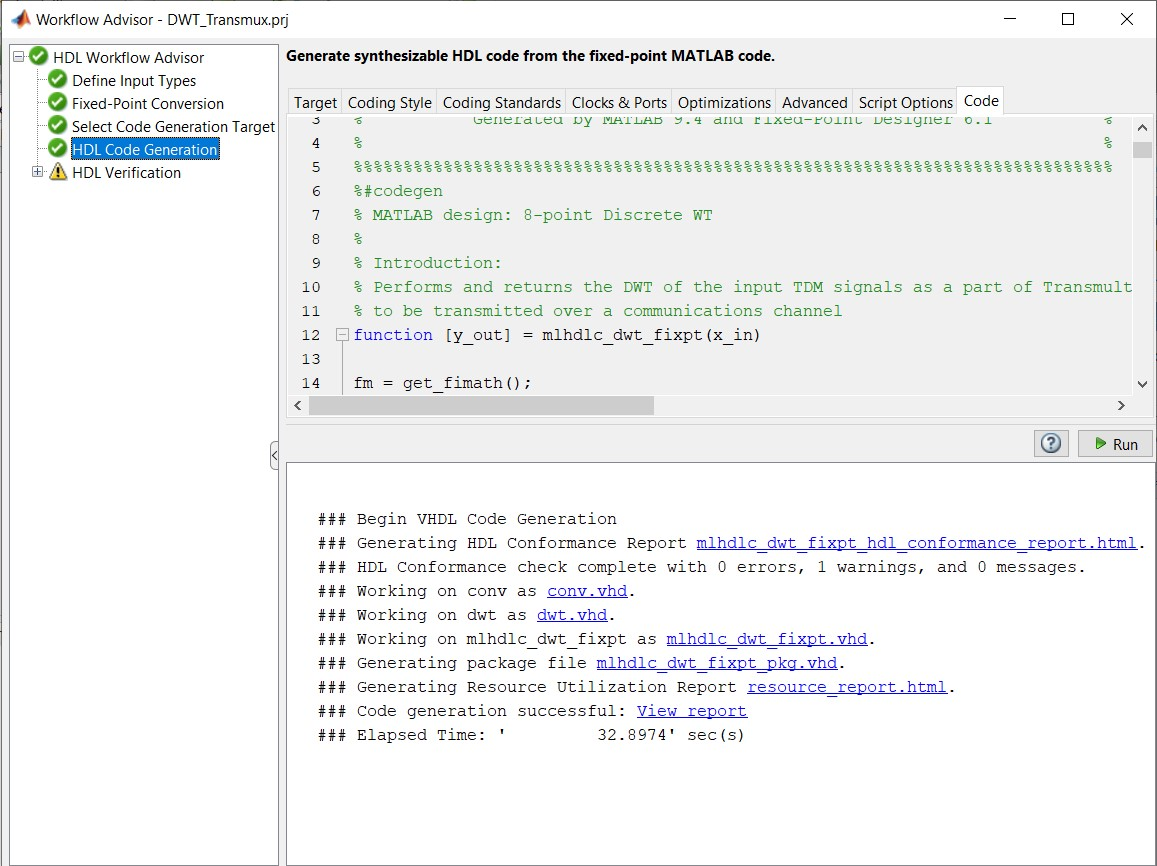
\includegraphics[width=170mm]{HDL_Coder.jpg}
    \caption{Output of HDL Code Generation.}
    \label{fig:hdl}
\end{figure}

\begin{table}[htpb]
    \centering
    \begin{tabular}{|c|c|c|}
    \hline
    System & Total Simulation Time & Processing Time \\
    \hline
         Proposed System (WT) & 36.43 s  & 1.43 s\\
         \hline
         Conventional System (FT) & 41.18 s & 6.18 s \\
         \hline
    \end{tabular}
    \caption{Time Complexity of the Proposed and Conventional System.}
    \label{tab:time}
\end{table}

\begin{figure}
    \centering
    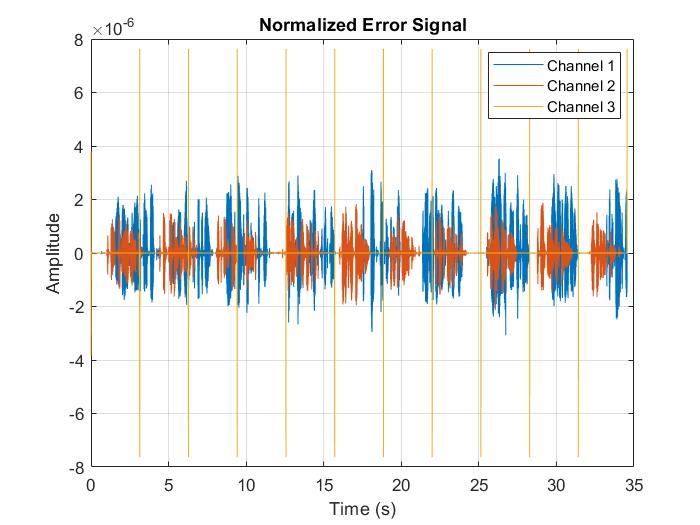
\includegraphics[width=110mm]{TestBench_Error.jpg}
    \caption{Normalized Error for the Test Bench Audio Signals.}
    \label{fig:test_bench_error}
\end{figure}

\newpage

\begin{figure}
    \centering
    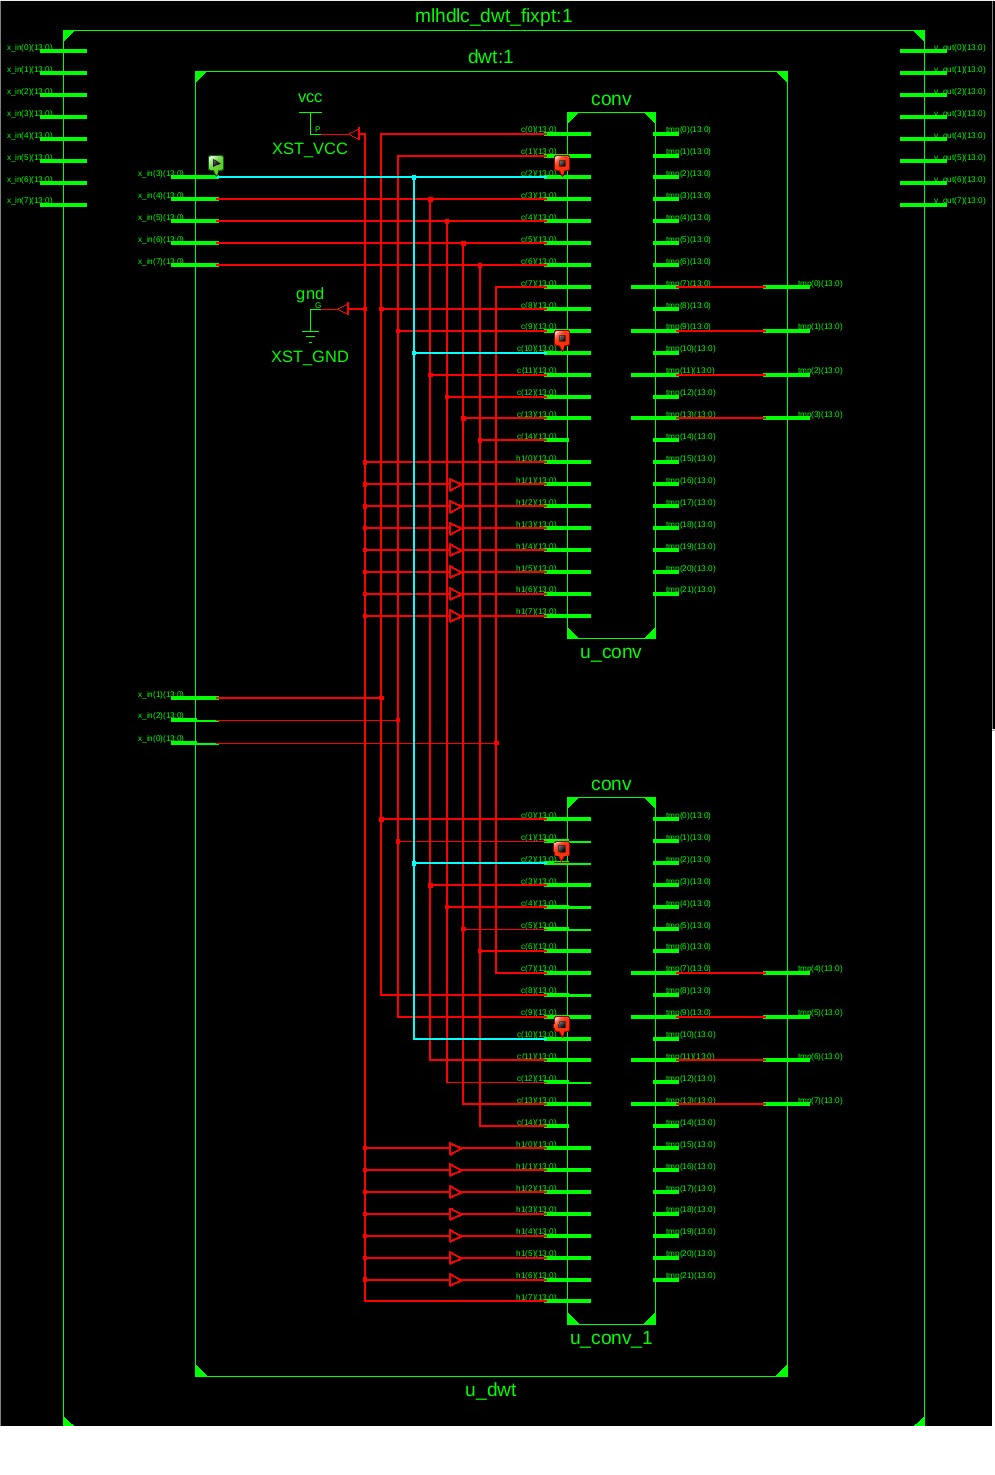
\includegraphics[width=156mm]{rtl_schematic.png}
    \caption{RTL Schematic of the Transmitter system.}
    \label{fig:rtl_transmitter}
\end{figure}

\section{Result Analysis}
This section discusses the results of the simulations obtained in this chapter. Table \ref{tab:sim},  highlights that the Designed Wavelet Filters improve upon the MSE by approximately 70 \% compared to other Wavelets for various channel models. It performs especially well under Rician fading channel conditions that characterize interference under LoS conditions, a useful metric for satellite systems \cite{channel}. Generic wavelets are constructed using predefined equations, which do not work well with filter bank-based systems. The designed filters perform better as they are specially designed for Trans-multiplexer systems and integrate well with the system requirements. Table \ref{tab:error_awgn} highlights the improvement in MSE for an AWGN channel achieved by the Wavelet-based Proposed system over the Fourier-based Conventional system. For low values of SNR, the performance of both systems is comparable. As the SNR values increase to about $-15$ dB, the Proposed system outperforms the Conventional system by a factor of approximately $10^{-4}$. The Proposed system exhibits better performance as it uses DWT and is able to extract both temporal and frequency information from the signals, allowing better reconstruction. For 15 dB of AWGN noise, the MSE of the simulated and emulated systems differed by 40.5 \%. Fig. \ref{fig:rtl_transmitter} shows the RTL Schematic of the transmitter generated using the VHDL code from the Coder.

The results of the simulation are apparent in the MATLAB HDL Coder Test Bench as well. The output audio signals at the receiver are clearly audible, showcasing perfect reconstruction. The Proposed system outperforms the Conventional system by a factor of approximately $10^{-3}$ in the HDL Test Bench. Table \ref{tab:time} highlights the improvement in time complexity achieved by the WT-based system. This is expected, as the time complexity of the WT-based system is $O(N)$ while that of FT-based system is $O(N*log(N))$. Thus, based on the various parameters discussed, it is apparent that the WT-based system is objectively better than Conventional FT-based systems, especially for satellite applications.
